\section{IntelliJ Idea configuration}

\begin{enumerate}
  \item Create a new project with \texttt{Jakarta EE} as generator:
    \begin{itemize}
      \item Template: web application
      \item JDK: OpenJDK 21 (path: \texttt{/usr/lib/jvm/java-21-openjdk})
      \item Build system: Maven\footnote{In accordance with the Software Engineering course.}
        \begin{figure}[H]
          \centering
          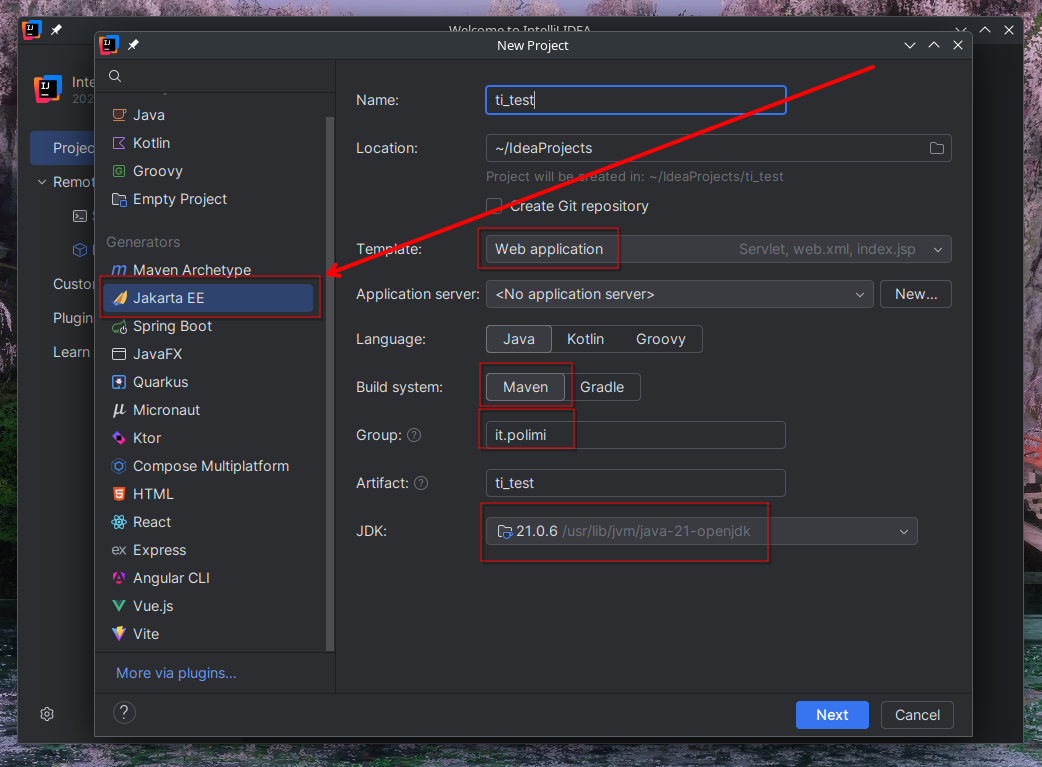
\includegraphics[width=0.6\textwidth]{img/intellij/intellij_2.png}
          \caption{IntelliJ project configuration.}
        \end{figure}

        % \newpage
      \item Application server: Tomcat (path: \texttt{/usr/share/tomcat10})
        \begin{figure}[H]
          \centering
          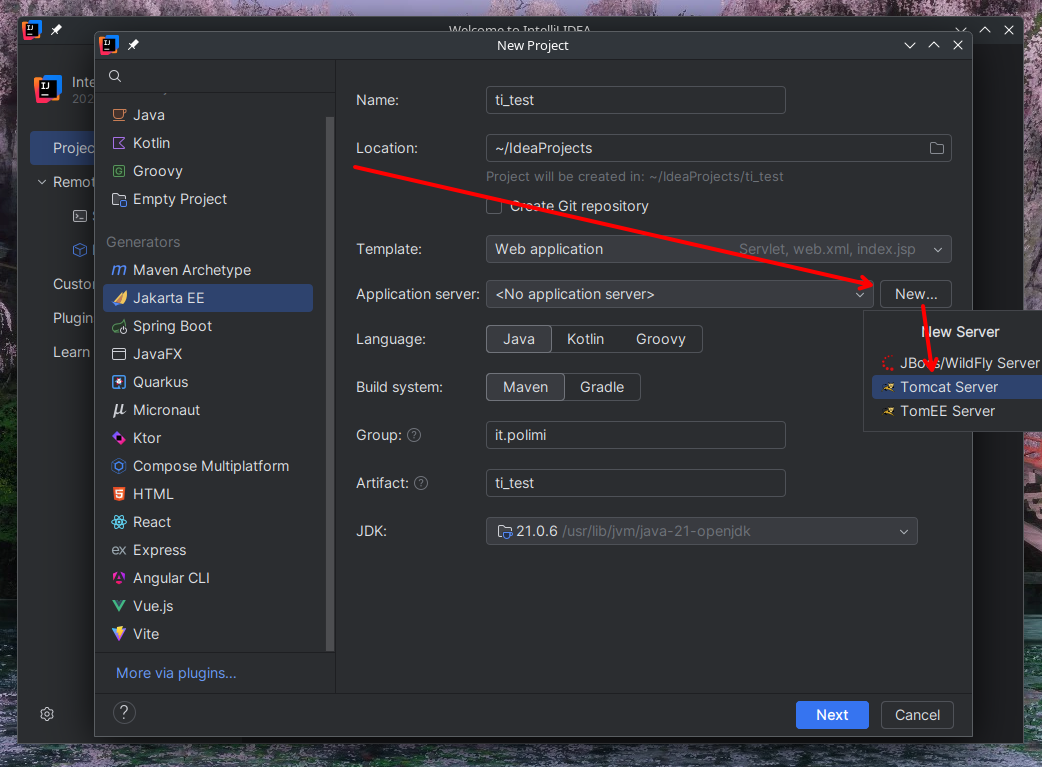
\includegraphics[width=0.6\textwidth]{img/intellij/intellij_3.png}
          \caption{Tomcat configuration (1/2).}
        \end{figure}

        \begin{figure}[H]
          \centering
          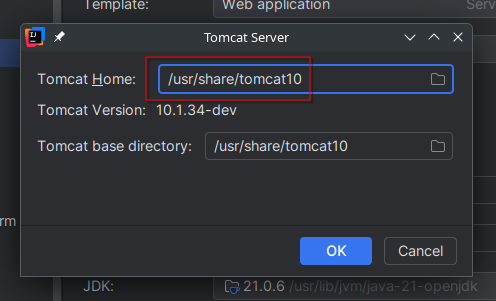
\includegraphics[width=0.45\textwidth]{img/intellij/intellij_4.png}
          \caption{Tomcat configuration (2/2).}
        \end{figure}
    \end{itemize}
  \item Check Eclipse server and client, Welde as implementations
    \begin{figure}[H]
      \centering
      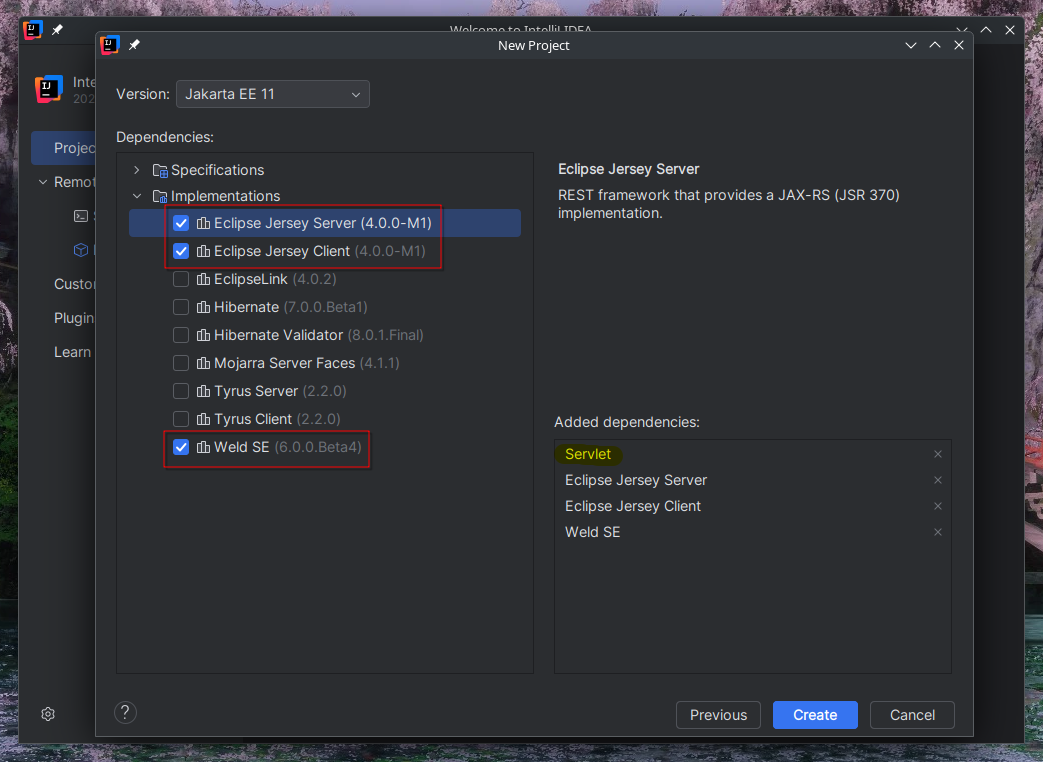
\includegraphics[width=0.6\textwidth]{img/intellij/intellij_5.png}
    \end{figure}
    Note that Servlet is already added as dependency.
\end{enumerate}

\begin{hint}[Permissions error]{}
  After a test, IntelliJ could report an error stating it cannot copy \texttt{/usr/share/tomcat10/conf} -- this maybe caused by permissions:
  \begin{figure}[H]
    \centering
    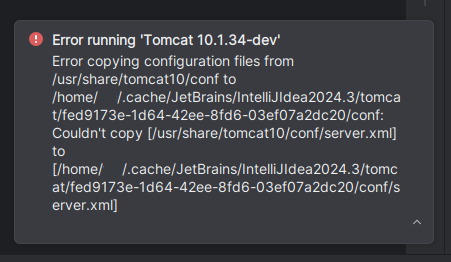
\includegraphics[width=0.5\textwidth]{img/intellij/intellij_6.png}
    \caption{IntelliJ error.}
  \end{figure}
  \newpage
  to fix it run:
    \begin{minted}{shell}
      sudo chmod -R 777 /usr/share/tomcat10/conf
    \end{minted}
\end{hint}

\subsection{Database configuration}\label{sec: db_intellij}

\begin{enumerate}
  \item Configure MariaDB
    \begin{minted}{shell}
    mariadb-install-db --user=mysql --basedir=/usr --datadir=/var/lib/mysql
    mariadb-secure-installation
    \end{minted}
    and then start it:
    \begin{minted}{shell}
    sudo systemctl start mariadb
    \end{minted}
    If you want to start the database server at every boot type:
    \begin{minted}{shell}
    sudo systemctl enable mariadb
    \end{minted}

  \item Create the user and grant \emph{all} permissions on \emph{all} databases:
    \begin{minted}{shell}
    sudo mariadb
    MariaDB [(none)]> CREATE USER 'name'@'localhost' IDENTIFIED BY 'password';
    MariaDB [(none)]> GRANT PRIVILEGES ON *.* TO 'name'@'localhost';
    MariaDB [(none)]> quit;
    \end{minted}
    this is needed since in order to create a database \emph{you need permission} to do so. If you want to verify:
    \begin{minted}{shell}
    MariaDB [(none)]> SHOW ALL PRIVILEGES FOR 'name'@'localhost';
    \end{minted}

  \item Open the database configuration from IntelliJ (above right)
    \begin{figure}[H]
      \centering
      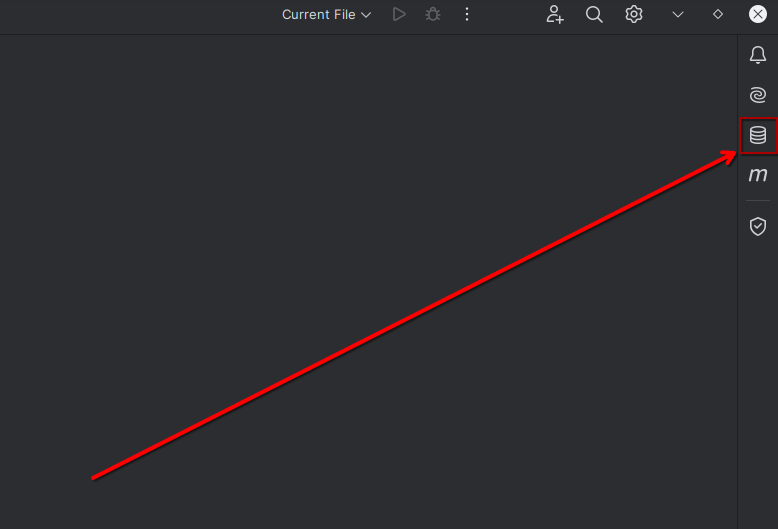
\includegraphics[width=0.6\textwidth]{img/intellij/intellij_8.png}
      \caption{Database configuration in IntelliJ.}
      \label{fig: intellij-db-config}
    \end{figure}

  \item To import a MySQL dump execute the following command:
    \begin{minted}{shell}
    mariadb --user name --password < dump.sql
    \end{minted}
    where \texttt{name} and \texttt{password} reference step 2.

    \newpage

  \item Add the data source from \autoref{fig: intellij-db-config}:
    \begin{itemize}
      \item Select MariaDB
        \begin{figure}[H]
          \centering
          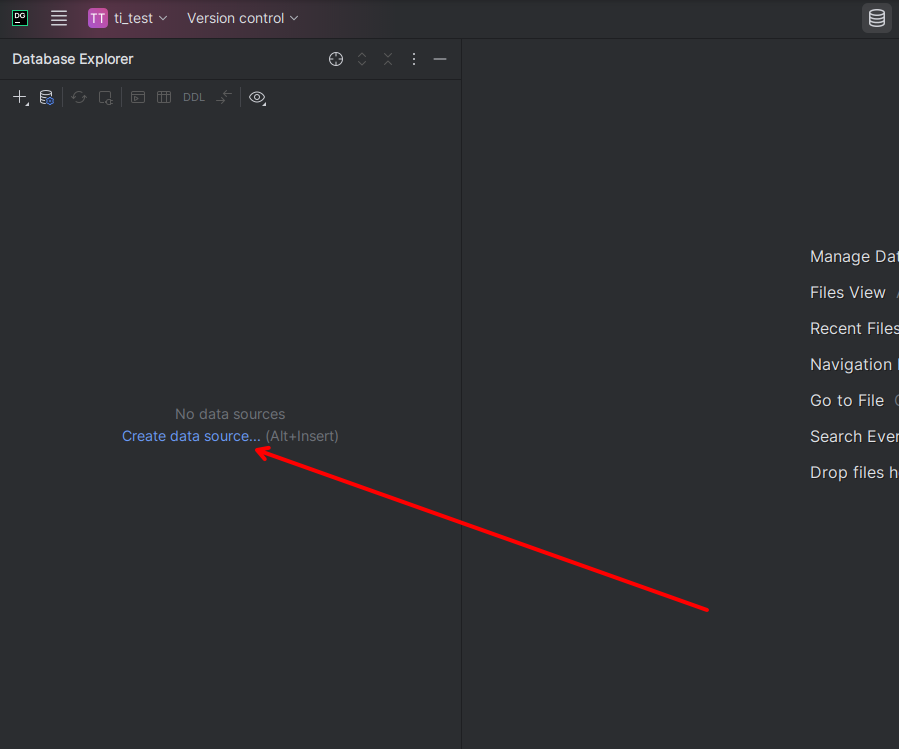
\includegraphics[width=0.49\textwidth]{img/datagrip/datagrip_2.png}
          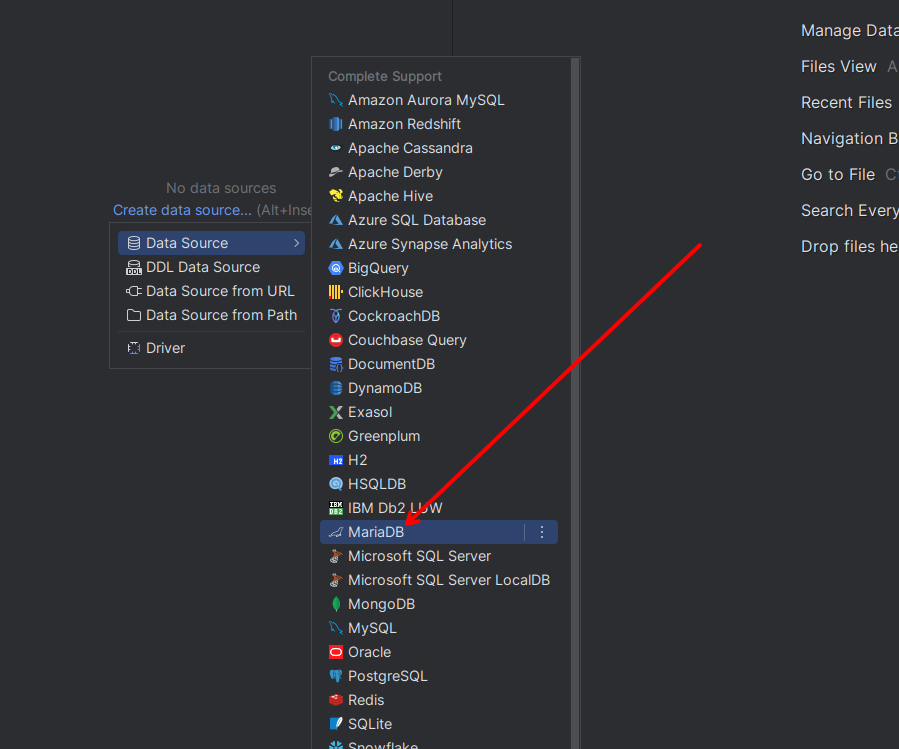
\includegraphics[width=0.49\textwidth]{img/datagrip/datagrip_3.png}
          \caption{Selecting MariaDB as source.}
        \end{figure}
      \item \texttt{user}, \texttt{password} from step 2
      \item Name of the database from step 5 -- to check available databases:
    \begin{minted}{shell}
    sudo mariadb
    MariaDB [(none)]> SHOW DATABASES;
    MariaDB [(none)]> quit;
    \end{minted}
    \end{itemize}
    \begin{figure}[H]
      \centering
      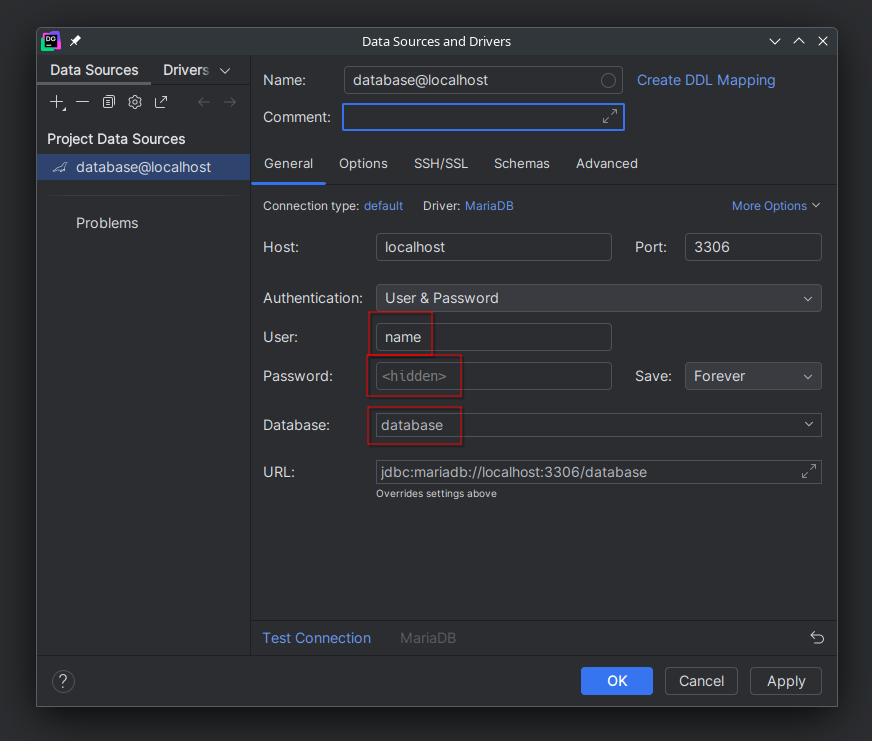
\includegraphics[width=0.6\textwidth]{img/datagrip/datagrip_4.png}
      \caption{Adding the database.}
    \end{figure}
\end{enumerate}

Repeat step 4 and 5 for each dump.

\newpage

\subsection{Configure MariaDB connection}

Add the following to \texttt{pom.xml}:
\begin{minted}{xml}
  <dependency>
   <groupId>org.mariadb.jdbc</groupId>
   <artifactId>mariadb-java-client</artifactId>
   <version>3.4.1</version>
  </dependency>
\end{minted}
and synchronize Maven, which then downloads all the necessary files. Last but not least, verify the connection by creating the \texttt{ConnectionTester} class:
\begin{minted}{java}
  import java.sql.*;

  public class ConnectionTester {
    public static void main(String[] args) throws SQLException,
    ClassNotFoundException {
      final String DATABASE = "database";
      final String USER = "name";
      final String PASSWORD = "password";
      Connection connection = null;

      // Load the JDBC driver
      try {
          Class.forName("org.mariadb.jdbc.Driver");
          System.out.println("Driver loaded");
      } catch (ClassNotFoundException e) {
          System.err.println("Driver not found");
          e.printStackTrace();
      }
      try {
          connection = DriverManager.getConnection
                  ("jdbc:mariadb://localhost:3306/" + DATABASE, USER, PASSWORD);
          System.out.println("Database connection successful");
          connection.close();
      } catch (Exception e) {
          System.err.println("Connection failed");
          e.printStackTrace();
      }
    }
  }
\end{minted}
by editing \texttt{DATABASE}, \texttt{USER} and \texttt{PASSWORD} accordingly.

\newpage

\subsection{Convert Eclipse projects}

Briefly the steps are:
\begin{enumerate}
  \item Figure out the dependencies and their versions
    \begin{itemize}
      \item This applies both to libraries (such as thymeleaf) and Java JDK
    \end{itemize}
  \item Paste the \texttt{/src} directory from the original project ZIP
  \item Add Tomcat run configuration
\end{enumerate}

Start by adding the dependencies to the \texttt{pom.xml}:
\begin{minted}{xml}
<dependencies>
    <!-- Jakarta EE servlet (jsp, jstl) -->
    <dependency>
        <groupId>org.glassfish.web</groupId>
        <artifactId>jakarta.servlet.jsp.jstl</artifactId>
        <version>2.0.0</version>
    </dependency>
    <dependency>
        <groupId>jakarta.servlet.jsp.jstl</groupId>
        <artifactId>jakarta.servlet.jsp.jstl-api</artifactId>
        <version>2.0.0</version>
    </dependency>
    <!-- Thymeleaf -->
    <dependency>
        <groupId>org.thymeleaf</groupId>
        <artifactId>thymeleaf</artifactId>
        <version>3.1.3.RELEASE</version>
    </dependency>
    <!-- Apache Commons -->
    <dependency>
        <groupId>org.apache.commons</groupId>
        <artifactId>commons-lang3</artifactId>
        <version>3.17.0</version>
    </dependency>
</dependencies>
\end{minted}

\begin{warning}[Pick the correct versions]{}
  \textbf{Be sure} to check for the correct versions. To do so, open the Eclipse's file \texttt{.classpath} and search in it. For example:
  {\scriptsize
  \begin{minted}{xml}
  <?xml version="1.0" encoding="UTF-8"?>
  <classpath>
    <classpathentry kind="con" path="org.eclipse.jdt.launching.JRE_CONTAINER/org.eclipse.jdt.internal.debug
    .ui.launcher.StandardVMType/JavaSE-21">
      <attributes>
        <attribute name="module" value="true"/>
      </attributes>
    </classpathentry>
    <classpathentry kind="src" path="src/main/java"/>
    <classpathentry kind="con" path="org.eclipse.jst.j2ee.internal.web.container"/>
    <classpathentry kind="con" path="org.eclipse.jst.j2ee.internal.module.container"/>
    <classpathentry kind="lib" path="src/main/webapp/WEB-INF/lib/apache-commons-lang.jar"/>
    <classpathentry kind="lib" path="src/main/webapp/WEB-INF/lib/mysql-connector-j-8.0.32.jar"/>
    <classpathentry kind="lib" path="src/main/webapp/WEB-INF/lib/attoparser-2.0.7.RELEASE.jar"/>
    <classpathentry kind="lib" path="src/main/webapp/WEB-INF/lib/javassist-3.29.0-GA.jar"/>
    <classpathentry kind="lib" path="src/main/webapp/WEB-INF/lib/ognl-3.3.4.jar"/>
    <classpathentry kind="lib" path="src/main/webapp/WEB-INF/lib/slf4j-api-2.0.16.jar"/>
    <classpathentry kind="lib" path="src/main/webapp/WEB-INF/lib/thymeleaf-3.1.3.RELEASE.jar"/>
    <classpathentry kind="lib" path="src/main/webapp/WEB-INF/lib/unbescape-1.1.6.RELEASE.jar"/>
    <classpathentry kind="con" path="org.eclipse.jst.server.core.container/org.eclipse.jst.server.tomcat
    .runtimeTarget/Apache Tomcat v10.1">
      <attributes>
        <attribute name="owner.project.facets" value="jst.web"/>
      </attributes>
    </classpathentry>
    <classpathentry kind="output" path="build/classes"/>
  </classpath>
  \end{minted}
  }
  If you look closely, you'll see that the dependencies of this project are:
  \begin{itemize}
    \item Java 21
    \item mysql-connector-j-8.0.3
    \item attoparser-2.0.7.RELEASE
    \item javassist-3.29.0-GA
    \item ognl-3.3.4
    \item slf4j-api-2.0.1
    \item thymeleaf 3.1.3.RELEASE
    \item unbescape-1.1.6.RELEASE
    \item Tomcat v10.1
  \end{itemize}
\end{warning}

And to set the JDK version:
\begin{minted}{xml}
    <properties>
        <!-- Properties set for Java 21 -->
        <maven.compiler.source>21</maven.compiler.source>
        <maven.compiler.target>21</maven.compiler.target>
        <project.build.sourceEncoding>UTF-8</project.build.sourceEncoding>
    </properties>
\end{minted}

Search them on the Maven repository with the following URL scheme:

\begin{center}
  \texttt{https://mvnrepository.com/artifact/\red{groupId}/\red{artifactId}}.
\end{center}

To build the application and deploy it you also need:
\begin{minted}{xml}
  <build>
      <plugins>
          <plugin>
              <artifactId>maven-compiler-plugin</artifactId>
              <version>3.13.0</version>
          </plugin>
          <plugin>
              <artifactId>maven-war-plugin</artifactId>
              <version>3.2.3</version>
          </plugin>
      </plugins>
  </build>
\end{minted}

Finally paste the \texttt{/src} directory from the desired project and configure Tomcat. An example can be seen in the \texttt{tomcat\_config.xml} file, which will have to be pasted into \texttt{.idea/run- Configurations} folder.

\begin{tip}[Optimize the conversion]{}
  Since these steps are the same for every project, I'd suggest to create a \texttt{template} folder which houses the \texttt{pom.xml} file along with the Tomcat configuration. This way, to convert a project you will only have to create a new directory and then paste in it the \texttt{src/} folder and the contents of \texttt{template}.
\end{tip}

\begin{warning}[Follow the standard structure]{}
  Finally, the directory tree will have to look like:
  \begin{verbatim}
    src/
    |-- main/
    |   |-- java/
    |   |   `-- it.polimi.tiw
    |   |-- resources
    |   `-- webapp
    `-- test/
        |-- java/
        |   `-- it.polimi.tiw
        |-- resources
        `-- webapp
    LICENSE.txt
    README.md
    pom.xml
  \end{verbatim}

  In accordance with the \href{https://maven.apache.org/guides/introduction/introduction-to-the-standard-directory-layout.html}{Maven standard directory layout}.

  This is \textbf{not optional}: for instance, in some projects there's a \texttt{resources} folder which is NOT located in the correct path; once the project will be deployed, Java will look for the \texttt{src/main/resources} folder and will not find it. IntelliJ won't throw an error.
\end{warning}
